\section{Heuristics for packing problems}

We now look at heuristics for the CLP.

\subsection{Wall-building}

This constructive heuristic was proposed by \textcite{GEORGE1980}, aiming to solve the CLP for a single container. In each iteration of the wall-building heuristic (WBH), what remains of the container is sliced by a plane parallel to its width and height, up to a certain depth. The resulting space is called a layer of the container.

\begin{figure}[h]
    \centering
    \begin{tikzpicture}[scale=0.5]
        \begin{scope}[fill=blue!20]
            \fill (0,0,0) -- (5,0,0) -- (5,0,-15) -- (0,0,-15) -- cycle;
            \fill (0,5,0) -- (5,5,0) -- (5,5,-15) -- (0,5,-15) -- cycle;
            \fill (0,0,-15) -- (5,0,-15) -- (5,5,-15) -- (0,5,-15) -- cycle;
            \fill (0,0,0) -- (5,0,0) -- (5,5,0) -- (0,5,0) -- cycle;
            \filldraw[dashed, pattern=north east lines, pattern color = red] (0,0,-4) -- (5,0,-4) -- (5,5,-4) -- (0,5,-4) -- cycle;
            \draw (0,0,0) -- (5,0,0) -- (5,5,0) -- (0,5,0) -- cycle;
            \draw (5,0,0) -- (5,0,-15);
            \draw (5,5,0) -- (5,5,-15);
            \draw (0,5,0) -- (0,5,-15);
            \draw (5,0,-15) -- (5,5,-15) -- (0,5,-15);
            \draw[dashed] (0,0,0) -- (0,0,-15);
            \draw[dashed] (0,5,-15) -- (0,0,-15) -- (5,0,-15);
            \draw[{|Stealth[length=2mm]}-{Stealth[length=2mm]|}] (5.5,0) -- (7,1.5);
            \node[right,black] at (7,0.75){\large{Layer depth}};
        \end{scope}
    \end{tikzpicture}
    \caption{Creation of a layer inside a container}
\end{figure}

To choose the depth of a new layer, we must first select a box, which we will call the layer's primary box. The primary box is selected as detailed in \cref{flow:primary box selection WBH}. Notice that we use the term ``box'' to refer to box types -- that is, the set of dimensions that define a box's volume. Hence, a box's ``quantity'' is the amount of boxes of said type that has yet to be packed.

\begin{figure}[h]
    \centering
    \begin{tikzpicture}[node distance=2cm]
        \node (start) [startstop] {Start};
        %\node (proc1) [process, below of=start] {Filter remaining boxes};
        \node (dec1) [decision, below of=start, align=center, yshift=-1cm, inner sep=-0.2ex] {Any remaining\\ box placed\\before?};
        \node (proc2) [process, left of=dec1, align=center, xshift=-4cm] {Select box according\\to ranking criteria};
        \node (proc3) [process, right of=dec1, align=center, xshift=4cm] {Select placed box\\with greatest\\quantity left};
        \node (end) [startstop, below of=dec1, yshift=-1cm] {Stop};

        \draw [arrow] (start) -- (dec1);
        %\draw [arrow] (proc1) -- (dec1);
        \draw [arrow] (dec1) -- node[anchor=south] {No} (proc2);
        \draw [arrow] (dec1) -- node[anchor=south] {Yes} (proc3);
        \draw [arrow,rounded corners=0.2cm] (proc2) |- (end);
        \draw [arrow,rounded corners=0.2cm] (proc3) |- (end);
    \end{tikzpicture}
    \renewcommand\figurename{Flowchart}
    \caption{Primary box selection procedure}
    \label[flowchart]{flow:primary box selection WBH}
\end{figure}

The ``ranking criteria'' in \cref{flow:primary box selection WBH} are as follows: First, we filter the boxes with the greatest smallest dimension. In case of ties, we filter the selected box with the greatest remaining quantity to pack. If ties persist, we choose one of the boxes with the greatest dimension. The intuition behind these choices is that it is better to pack larger items first, to avoid complications trying to fit them with smaller items later on. It is also preferable to pack numerous boxes first, in order to reduce their numbers quickly.

Layers provide an initial space into which boxes can be placed. For this initial space, the chosen box to start the filling process is the primary box, since it can be rotated to perfectly fit the space's depth. Once this space is filled with as many primary boxes as possible, certain unfilled spaces might remain. \cref{fig:remaining spaces first filling WBH A} illustrates this situation. The two spaces on top of the boxes are called height-wise spaces, while the space to the right is called width-wise space. If, for example, we fill any of the remaining spaces, new unfilled spaces might appear. \cref{fig:remaining spaces first filling WBH B} shows this situation. Notice that an unfilled space in front of the filling appears -- this is called a depth-wise space.

\begin{figure}[h]
    \centering
    \begin{subfigure}{.45\textwidth}
        \centering
        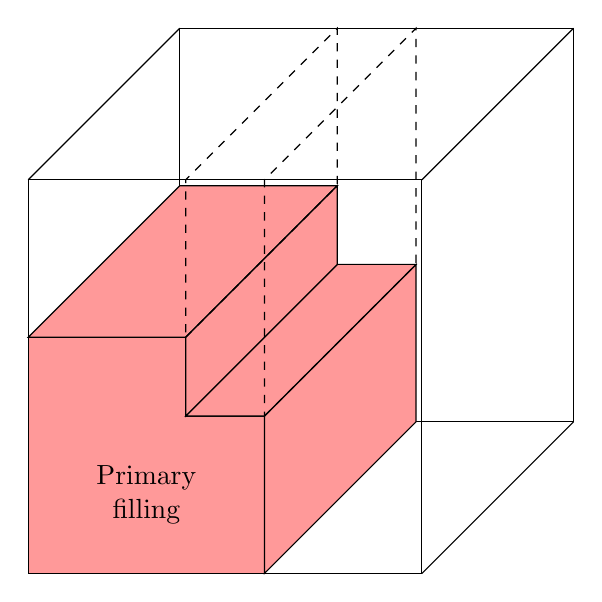
\begin{tikzpicture}[scale=0.5]
            \begin{scope}[fill=red!40]
                \draw (0,0,0) rectangle (10,10,0);
                \draw (0,0,-10) rectangle (10,10,-10);
                \draw (10,0,0) -- (10,0,-10);
                \draw (10,10,0) -- (10,10,-10);
                \draw (0,10,0) -- (0,10,-10);
                \filldraw (0,6,0) -- (0,6,-10) -- (4,6,-10) -- (4,6,0) -- cycle;
                \filldraw (0,0,0) -- (6,0,0) -- (6,4,0) -- (4,4,0) -- (4,6,0) -- (0,6,0) -- cycle;
                \filldraw (6,0,0) -- (6,0,-10) -- (6,4,-10) -- (6,4,0) -- cycle;
                \filldraw (6,4,0) -- (6,4,-10) -- (4,4,-10) -- (4,4,0) -- cycle;
                \filldraw (4,4,-10) -- (4,6,-10) -- (4,6,0) -- (4,4,0) -- cycle;
                \draw[dashed] (4,6,0) -- (4,6,-10) -- (4,10,-10) -- (4,10,0) -- cycle;
                \draw[dashed] (6,4,0) -- (6,4,-10) -- (6,10,-10) -- (6,10,0) -- cycle;
                \node[align=center] at (3,2) {Primary\\filling};
            \end{scope}
        \end{tikzpicture}
        \caption{Unfilled spaces around primary filling}
        \label{fig:remaining spaces first filling WBH A}
    \end{subfigure}
    \begin{subfigure}{.45\textwidth}
        \centering
        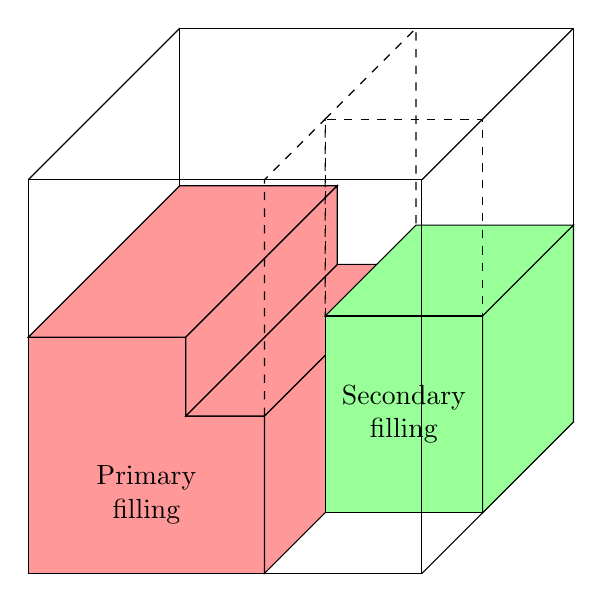
\begin{tikzpicture}[scale=0.5]
            \begin{scope}[fill=red!40]
                \draw (0,0,0) rectangle (10,10,0);
                \draw (0,0,-10) rectangle (10,10,-10);
                \draw (10,0,0) -- (10,0,-10);
                \draw (10,10,0) -- (10,10,-10);
                \draw (0,10,0) -- (0,10,-10);
                \filldraw (0,6,0) -- (0,6,-10) -- (4,6,-10) -- (4,6,0) -- cycle;
                \filldraw (0,0,0) -- (6,0,0) -- (6,4,0) -- (4,4,0) -- (4,6,0) -- (0,6,0) -- cycle;
                \filldraw (6,0,0) -- (6,0,-10) -- (6,4,-10) -- (6,4,0) -- cycle;
                \filldraw (6,4,0) -- (6,4,-10) -- (4,4,-10) -- (4,4,0) -- cycle;
                \filldraw (4,4,-10) -- (4,6,-10) -- (4,6,0) -- (4,4,0) -- cycle;
                \node[align=center] at (3,2) {Primary\\filling};
            \end{scope}
            \begin{scope}[fill=green!40]
                \filldraw (6,5,-4) -- (6,5,-10) -- (10,5,-10) -- (10,5,-4) -- cycle;
                \filldraw (10,0,-4) -- (10,0,-10) -- (10,5,-10) -- (10,5,-4) -- cycle;
                \filldraw (6,0,-4) -- (10,0,-4) -- (10,5,-4) -- (6,5,-4) -- cycle;
                \draw (10,0,0) -- (10,10,0);
                \draw[dashed] (6,5,-4) -- (6,10,-4) -- (10,10,-4) -- (10,5,-4);
                \draw[dashed] (6,10,-4) -- (6,10,-10) -- (6,5,-10);
                \draw[dashed] (6,4,0) -- (6,10,0) -- (6,10,-4) -- (6,5,-4);
                \node[align=center] at (8,2.5,-4) {Secondary\\filling};
            \end{scope}
        \end{tikzpicture}
        \caption{Unfilled spaces around secondary filling}
        \label{fig:remaining spaces first filling WBH B}
    \end{subfigure}
    \caption{Remaining spaces in the first filling of a layer}
    \label{fig:remaining spaces first filling WBH}
\end{figure}

To figure out whether a space should be stored in memory for filling, we only need to check if its height or its width (in the case of a height- or width-wise space, respectively) is greater than the smallest dimension of any remaining box. Depth-wise spaces are created regardless of any such check, because they may be \emph{amalgamated} later on. For example, consider the top view of two layers in \cref{fig:amalgamation example}. The previous layer was packed with two depth-wise spaces left unfilled. We select the depth-wise space with minimal depth to amalgamate with the space in the current layer. The original space is reduced to space $A$, with the amalgam $B \cup C$ to its right. Space $B$ is defined by a \emph{flexible width} parameter, which allows the algorithm to fill space $A$ past its boundaries, as long as its last column of boxes is both in $A$ and $B$, but not in $C$. In such circumstances, the width of $A$ is increased and the width of the amalgam is decreased according to the length of flexible width consumed by this last column of boxes.

\begin{figure}[h]
    \centering
    \begin{tikzpicture}
        \fill[dashed,pattern=north east lines, pattern color=green!80] (0,0) rectangle (3,2);
        \fill[dashed,pattern=north east lines, pattern color=red!80] (3,0) rectangle (4.5,2.5);
        \fill[dashed,pattern=north east lines, pattern color=yellow!80] (4.5,0) rectangle (9,2.5);
        \filldraw[fill=blue!40] (0,2) -- (3,2) -- (3,2.5) -- (5,2.5) -- (5,3.5) -- (9,3.5) -- (9,5) -- (0,5) -- cycle;
        \draw[{|Stealth[length=2mm]}-{Stealth[length=2mm]|}] (-0.3,2) -- (-0.3,5);
        \draw[{|Stealth[length=2mm]}-{Stealth[length=2mm]|}] (-0.3,0) -- (-0.3,2);
        \node[anchor=east, align=center] at (-0.3,3.5) {Previous\\layer};
        \node[anchor=east, align=center] at (-0.3,1) {Current\\layer};
        \draw[dashed] (5,2.5) -- (9,2.5);
        \draw[{|Stealth[length=2mm]}-{Stealth[length=2mm]|}] (9.3,0) -- (9.3,2.5);
        \node[anchor=west, align=center] at (9.3,1.25) {Amalgam\\depth};
        \draw (0,0) rectangle (9,5);
        \draw[{|Stealth[length=2mm]}-{Stealth[length=2mm]|}] (0,-0.3) -- (3,-0.3);
        \node[anchor=north, align=center] at (1.5,-0.3) {Min. original\\space width};
        \draw[{|Stealth[length=2mm]}-{Stealth[length=2mm]|}] (3,-0.3) -- (4.5,-0.3);
        \node[anchor=north, align=center] at (3.75,-0.3) {Flexible\\width};
        \draw[{|Stealth[length=2mm]}-{Stealth[length=2mm]|}] (4.5,-0.3) -- (9,-0.3);
        \node[anchor=north, align=center] at (6.75,-0.3) {Min. amalgam\\width};
        \node[draw,circle] at (1.5,1) {\large{A}};
        \node[draw,circle] at (3.75,1) {\large{B}};
        \node[draw,circle] at (6.75,1) {\large{C}};
    \end{tikzpicture}
    \caption{Amalgamation procedure}
    \label{fig:amalgamation example}
\end{figure}

It should be noted that in this example we assume the depth-wise space chosen is at the same height or lower than the current layer's space. Otherwise, it does not make sense to attempt to amalgamate them.

Finally, we discuss this heuristic's packing method. First, we determine if a space can be filled by filtering the box rotations that fit in it. If there is any, then there are two scenarios:

\begin{enumerate}
    \item There are box rotations whose width is at most half of the space's width: Choose one such box with maximum depth.
    \item Otherwise: Choose a box rotation with maximum width-by-depth area.
\end{enumerate}

Both selections try to minimize the unused base area of the space. In particular, the logic behind scenario 1 is that such boxes can be stacked in columns side by side, so we count the width-by-depth area of all the columns of boxes. After making the selection, we fill the space according to \cref{flow:space filling procedure WBH}.

\begin{figure}[h]
    \centering
    \begin{tikzpicture}
        \node (start) [startstop] {Start};
        \node (dec1) [decision,below of=start,yshift=-2cm] {Can width\\and height be\\swapped?};
        \node (proc1) [process,below of=dec1,align=center,yshift=-2cm] {Keep current\\rotation};
        \node (dec2) [decision,right of=dec1, inner sep=-0.1,xshift=3.5cm] {Can complete\\a column with\\either rotation?};
        \node (proc2) [process,right of=dec2,xshift=3.5cm] {Choose rotation\\that maximizes\\column height};
        \node (proc3) [process,below of=dec2,yshift=-2.5cm] {Choose larger\\dimension as\\width};
        \node (proc4) [process,below of=proc1, yshift=-4cm] {Pack column};
        \node (dec3) [decision,right of=proc4,xshift=3cm] {Column\\within flexible\\width?};
        \node (dec4) [decision,below of=dec3, yshift=-3cm] {Are there\\still boxes of\\this type?};
        \node (dec5) [decision,left of=dec4,xshift=-3cm] {Enough\\space for new\\column?};
        \node (end) [startstop, right of=dec3, xshift=3.5cm] {Stop};

        \draw [arrow] (start) -- (dec1);
        \draw [arrow] (dec1) -- node [anchor=south] {Yes} (dec2);
        \draw [arrow] (dec1) -- node [anchor=east] {No} (proc1);
        \draw [arrow] (dec2) -- node [anchor=south] {Yes} (proc2);
        \draw [arrow] (dec2) -- node[anchor=east] {No} (proc3);
        \draw [arrow] (proc1) -- (proc4) node [midway] (M) {};
        \draw [arrow, rounded corners=0.2cm] (proc2) |- (M.center);
        \draw [arrow, rounded corners=0.2cm] (proc3) |- (M.center);
        \draw [arrow] (proc4) -- (dec3);
        \draw [arrow] (dec3) -- node[anchor=east] {No} (dec4);
        \draw [arrow] (dec4) -- node[anchor=south] {Yes} (dec5);
        \draw [arrow] (dec5) -- node[anchor=east] {Yes} (proc4);
        \draw [arrow] (dec3) -- node [anchor=south] {Yes} (end) node [midway] (N) {};
        \draw [arrow, rounded corners] (dec4.east) -- node [anchor=south] {No} (dec4 -| end) -- (end.south);
        \draw [arrow, rounded corners] (dec5.south) -- node [anchor=east] {No} ([yshift=-0.5cm]dec5.south) -- ([yshift=-0.5cm]dec5.south -| end) -- (end.south);
    \end{tikzpicture}
    \caption{Space filling procedure}
    \renewcommand\figurename{Flowchart}
    \label[flowchart]{flow:space filling procedure WBH}
\end{figure}